\documentclass[twocolumn,preprintnumbers,amsmath,amssymb,superscriptaddress]{revtex4}
%\usepackage[pdftex]{graphicx}

\usepackage{amsmath,amsfonts,amssymb}
\usepackage[english]{babel}
\usepackage[latin1]{inputenc}
\usepackage[T1]{fontenc}
\usepackage{color}
\usepackage{float}
\usepackage{verbatim}
\usepackage{graphicx}
\usepackage{bm}
\usepackage{mathtools}
\usepackage{stmaryrd}
\usepackage{anyfontsize}

\usepackage[font={small}]{caption}
\usepackage{subcaption}
\captionsetup{compatibility=false}

%\usepackage{epstopdf}
%\usepackage{array}
%\usepackage{tabularx}
%\usepackage{multirow}
\usepackage{color}
%\usepackage{multibox}
%\usepackage{rotating}
%\usepackage{lineno}
%\usepackage[left]{lineno}
%\usepackage[comma,sort&compress]{natbib}
%\usepackage{authblk}
%\usepackage{multicol}

\bibliographystyle{ieeetr}

\usepackage{bibunits}

\newcommand{\beginsupplement}{%
        \clearpage
        \setcounter{table}{0}
        \renewcommand{\thetable}{S\arabic{table}}%
        \setcounter{figure}{0}
        \renewcommand{\thefigure}{S\arabic{figure}}%
     }


%\linenumbers
%\setlength\linenumbersep{3pt}

\begin{document}


%\title{Simple rules yield complex communities: deconstructed species interactions and the assembly of communities}
%\title{Community assembly and dynamics by the deconstruction of species interactions}
\title{Lost in space: the eco-evolutionary impacts of straying on metapopulation robustness}
\author{Justin D. Yeakel${}^{1,2,*}$, Jean Philippe Gibert${}^{1}$, Peter Westley${}^{3}$, \& Jonathan W. Moore${}^{4}$ \\
${}^1$School of Natural Sciences, University of California, Merced, Merced CA, USA \\
${}^2$The Santa Fe Institute, Santa Fe NM, USA \\
${}^3$College of Fisheries and Ocean Sciences, University of Alaska, Fairbanks, Fairbanks AK, USA \\
${}^4$Earth${}_2$Oceans Research Group, Simon Fraser University, Vancouver BC, Canada \\
${}^*$To whom correspondence should be addressed: jdyeakel@gmail.com
}



\maketitle



\section{Introduction}


%Motivation: straying
Coordinated mass migrations are one of the great wonders of the natural world, and the ability of individuals and groups to navigate across great distances have long fascinated naturalists \cite{MilnerGulland:2011vm}.
Anadromous salmonid fishes (genera \emph{Oncorhynchus} and \emph{Salmo}) embody these astonishing migrations by homing with high accuracy and precision to their natal streams for reproduction after years at sea \cite{Quinn:2011tf,Jonsson:2011kg,Keefer:2014gg}.
Nothwithstanding their philopatric tendancy, not all individuals home, but rather `stray' to non-natal sites to spawn \cite{Quinn:1993ge,Hendry:2004wf,H:2013fs}.
Although extensive work has been done to document the extent of straying from donor populations and into recipient populations \cite{Keefer:2014gg,Bett:2017ha}, only recently have the abiotic, biotic, and anthropogenic influences of `straying' behaviors been investigated systemically \cite{Keefer:2008bs,Westley:2015to,Bond:2016dz}.
Most recently the role of social interactions and collective navigation has been hypothesized \cite[][; this volume]{Berdahl:2015kv,Berdahl:2016dx}.
Although the straying of individuals into sites hosting other populations provides connections within the larger metapopulation, potentially promoting ecological and evolutionary rescue, it also serves to introduce maladapted individuals into habitats that are host to different environmental conditions, and this may lower the mean fitness of the local (mixed) population \cite{Muhlfeld:2014hs}.



%The tradeoff
The dual nature of straying as both promoter of connections among metapopulation demes and potential eroder of locally adapted gene complexes highlights the interplay between ecological dynamics of connected populations as well as the evolutionary dynamics of mixed trait distributions that respond to alternative local conditions.
Population-level biodiversity is recognized to increase species persistence (REFS), and the resilience and sustainability of metapopulations (general REF).
For example, the long-term sustainability of the Bristol Bay sockeye salmon fishery is due in large part to intact habitat that in conjunction with fine-scale homing and reduced gene flow provides a template for the evolution of countless locally adapted populations \cite{Hilborn:2003gf,Schindler:2010he,Anonymous:2014ku,Satterthwaite:2015ge}.
In contrast, areas such as California's Central Valley where habitats have been lost, degraded, and homogenized stand in marked contrast.
Within species diversity (or lack thereof) can manifest itself by way of asynchronous population dynamics, where the drivers that give rise to changes in population size vary across a metapopulation, decreasing the potential for synchronization, and correspondingly increasing the potential for ecological rescue (REFS).
This statistical buffer against extinction has traditionally been quantified as the Portfolio Effect (PE), which is the ratio of the population CV to the CV of the aggregated metapopulation.
Weakened portfolio dynamics can also emerge from homogenization resulting from  reduced genetic variability among populations, where homogenous stocks are more likely to have similar life-history structures (REFS), be at greater risk disease-induced epidemics (REFS), and recruit sub-optimally in heterogeneous environments (REFS).
Of course, these two measures of diversity often occur concurrently: for instance, lower genetic diversity increases the likelihood that two populations respond similarly to the same stressors, and this promotes synchronized dynamics, thus lowering portfolio effects.

%Eco-evolutionary dynamics in space
%% From geographic mosaic of coevolution to...
That evolutionary forces play out heterogeneously across geographic mosaics is now a foundational concept in ecology and evolutionary biology (REFS).
These mosaics are in part driven by environmental differences between habitats that alter the selective forces acting on different phenotypes \cite{Endler:1986tz}, and a principle underlying assumption is that there is gene flow such that individuals from different habitats mix over space (REFS).
Although the evolutionary outcomes of these spatial processes have been explored in depth (REFS), it is less well understood how selective mosaics and their consequent evolutionary forces impact population dynamics over contemporary timescales \cite{Hendry:2016un}.
How the ecological dynamics of phenotypically diverse metapopulations, wherein constituent populations are subject to different selective regimes, are altered affected by evolutionary forces is less well known. % and the subject of this paper.

%Movement through space (link back to straying)
Migratory populations that return to a breeding ground or natal stream to reproduce are linked to each other by some proportion of the population that permanently disperse, or stray into the `wrong' site; we might say that there is at least one \emph{Kevin} in every school or flock in every school or flock (figure \ref{fig:xkcd}).
The rate at which individuals stray, $m$, has been subject to a growing amount of both theoretical and empirical research \cite{H:2013fs,Keefer:2014gg,Bett:2017ha} and may be linked to errors made at an individual-level that are themselves diminished by migrating in groups and pooling individual choices \cite{Berdahl:2015kv,Berdahl:2016dx}.
Regardless of the mechanism's governing straying, the effect that it has on the dynamics of individual populations and the metapopulation as a whole is a topic of considerable interest that has tangible conservation implications \cite{Brenner:2012gl,Johnson:2012fe,Fullerton:2011ii}.
Whether, and to what extent, the ecological consequences of straying depend on the evolutionary dynamics that emerge from populations distributed across a selection mosaic is unclear.
How the assumed negative evolutionary effects of straying and subsequent gene flow is balanced by the positive effects of demographic rescue is the subject of this contribution.

%Here we show: pattern formation, dependence on heritability, large effects of small amounts of straying

\begin{figure}
  \captionsetup{justification=raggedright,
singlelinecheck=false
}
\centering
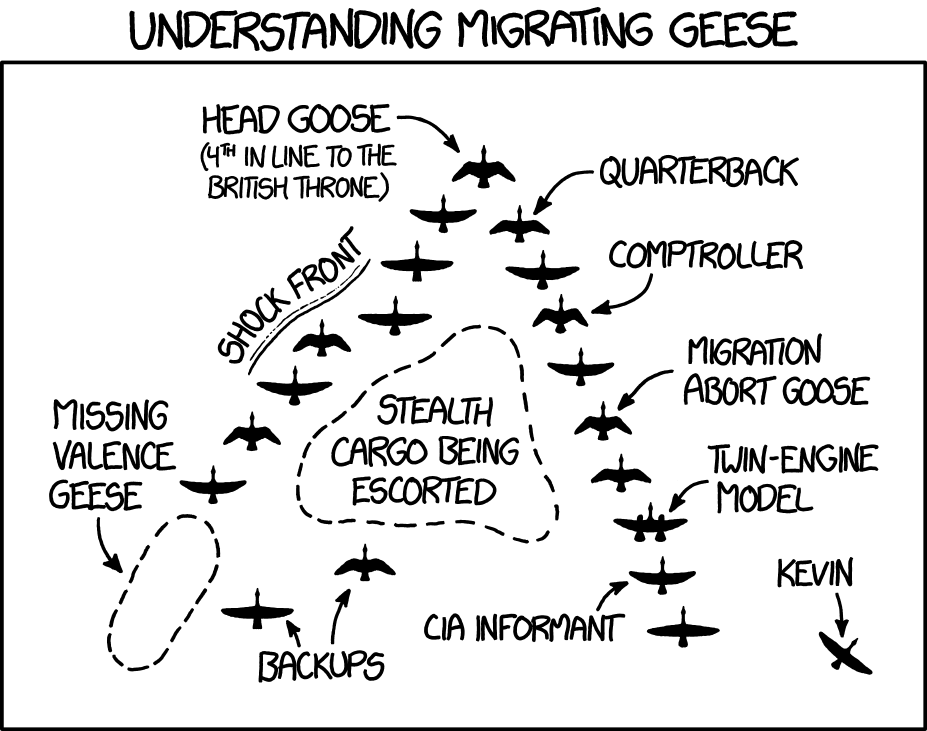
\includegraphics[width=0.4\textwidth]{figs2/fig_xkcd.png}
\caption{
\emph{Migrating Geese}, a comic from Randall Monroe's xkcd (https://xkcd.com/1729/). 
A flock of geese travel in the direction of a shared destination, the lone stray named \emph{Kevin}.
In this case, the rate of straying is $m=0.05$, which is not an uncommon rate for migrating populations of salmon \cite{Satterthwaite:2015ge}. 
Reprinted under the Creative Commons Attribution-NonCommercial 2.5 License.
} \label{fig:xkcd}
\end{figure}

%Alternative stable state
Here we ask the overarching question: how does collective behavior mediated dispersal and gene flow interact to influence the robustness of locally adapted populations?
To address this question we construct a minimal eco-evolutionary model of two populations occupying different sites that are linked by straying individuals, each of which with an associated trait distribution subject to natural selection determined by local conditions.
An important and relatively novel component of this model is the inclusion of a parameter that defines the difference in local conditions that favor different trait optima, increasing values of which correlates to populations that mix across increasingly heterogeneous environments \cite[though see ]{Berdahl:2015kv}.
Although our proposed model is was constructed with the dynamics of salmon populations in mind, the framework is general and the conclusions are likely relevant to a diverse range of migratory organisms where locally adapted populations are linked by dispersal.
We first show that specific rates of straying and trait heritability can have large effects on the qualitative dynamics of populations over time, in many cases giving rise to alternative steady states where one site is pushed towards very low biomass.
The emergence of alternative steady states results in a nonlinear response of the portfolio effect as well as the time required for the metapopulation to recover after an induced disturbance, suggesting that metapopulation robustness can be quite sensitive to the combined influences of dispersal across a selective landscape.

%Extinction and return times

%Habitat heterogeneity
A second important finding of our minimal model reveals that systems with greater habitat heterogeneity (measured by an increased difference in the trait values that are optimal between sites) host an intermediate range of straying rates where the portfolio effect increases to a local maximum, signaling that under certain conditions moderate amounts of straying between populations can increase the likelihood of persistence despite the deleterious evolutionary effects overall.
However, if we suppose that the rate of straying between two sites is correlated with distance (as indicated by empirical evidence), and that the difference in trait optima increases with distance as would be the case if the optima were associated with alternative temperature regimes (especially if sites are distributed latitudinally rather than longitudinally), even a very small amount of straying can drastically reduce the portfolio effect.
Importantly, the qualitative nature of our results do not depend on whether the stray rate is density dependent or constant, suggesting a limited role of collective dispersal on the dynamics considered herein.

%Concluding paragraph of the intro




\section{Model Description \& Analysis}

\noindent{\bf (a) Metapopulation framework}\\
\noindent We consider two populations $N_1$ and $N_2$ that are separated in space in distinct habitats, each with trait values $x_1$ and $x_2$ determining recruitment rates.
We assume that there is an optimum trait value $\theta_1$ and $\theta_2$ associated with each habitat, where recruitment is maximized if the trait value of the local population $x = \theta$.
Moreover, we assume that $x_{1,2}$ are normally distributed with means $\mu_1$ and $\mu_2$ and have the same standard deviation $\sigma$.
As such, the recruitment rate for both populations is determined by the mean trait value of the local population, such that $r_1 = R_1[\mu_1(t),\theta_1]$.
Trait means for each population are subject to selection, the strength of which depends on the difference between the population mean and the local trait optimum at a given point in time \cite{simpson1953major,Lande:1976ga}.

The two populations are assumed to reproduce in spatially separate sites that are close enough such that a proportion of the population $m$ can stray into the other site, and where mortality occurs before individuals return to reproduce.
If there is no straying between these populations (such that they are independent), then the mean trait evolves towards the optimal value such that $x_1 \rightarrow \theta_1$, and the recruitment rate for that population will be maximized.
If there is straying between populations at rate $m$, then the traits in each respective location will be pulled away from the optimum, and recruitment rates will be lowered.
As $m \rightarrow 0.5$, the populations are perfectly mixed, acting as a single population.

\begin{figure}
  \captionsetup{justification=raggedright,
singlelinecheck=false
}
\centering
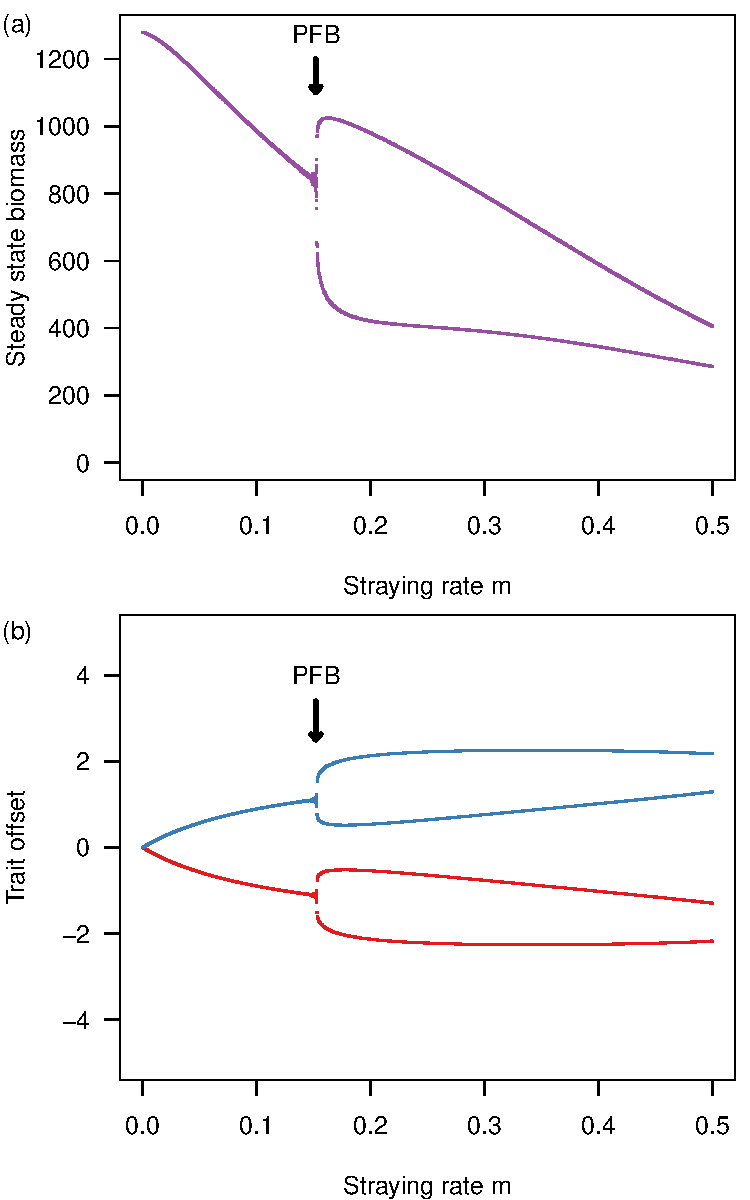
\includegraphics[width=0.4\textwidth]{figs2/fig_traj.pdf}
\caption{
A) The steady state densities of $N_1$ and $N_2$ as a function of a constant stray rate $m$. Which population attains the low- or high-density state is random due to small applied fluctuations in the initial conditions.
B) The steady state trait values measured as $\theta_i - x_i$, as a function of a constant stray rate $m$. 
} \label{fig:traj}
\end{figure}

We use the discrete Ricker population dynamic framework described by Shelton and Mangel \cite{Shelton:2011eq} as the basis for our two-site model, with the added effect of the local population $N_i$ mixing with a set proportion $m$ of a remote population $N_j$ that is straying into it.
In this sense, both populations serve as donor and recipient populations.
We first assume that the proportion ${\rm e}^{-Z}$ of both populations survive such that the surviving aggregated population, composed of both local individuals (at site $i$) and incoming strays (from site $j$), is $\left((1-m)N_i(t) + m N_j(t) \right){\rm e}^{-Z}$.
Because local individuals will recruit differently than incoming strays, the recruitment of the aggregate must incorporate two recruitment functions, given by $\left(R_i[\mu_i(t)] (1-m)N_i(t) + R_i[\mu_j(t)] m N_j(t)\right)$.
This mix of individuals is subject to the same compensatory effects, which is determined by the parameter $\beta$.
Taken together, the difference equation that determine changes in population size is

\begin{align}
  &N_i(t+1) = \\ \nonumber
  &\left((1-m)N_i(t) + m N_j(t) \right){\rm e}^{-Z} \\ \nonumber
  &+ \left(R_i[\mu_i(t)] (1-m)N_i(t) + R_i[\mu_j(t)] m N_j(t)\right) \\ \nonumber
  &\times {\rm e}^{-\beta ((1-m)N_i(t) + m N_j(t))},
  \label{eq:N}
\end{align}

\noindent where the difference equation for $N_j$ mirrors that for $N_i$.

The combined recruitment of local individuals $(1-m)N_i(t)$ and incoming strays $mN_j(t)$, as a function of their mean trait value at time $t$.
Given the local trait optimum is $\theta_i$, recruitment is

\begin{align}
  &R_i[\mu_i(t)] = \\ \nonumber
  &\int_{-\infty}^\infty r_{\rm max}\exp\left\{\frac{(x_i(t)-\theta_i)^2}{2\tau^2}\right\} {\rm pr}(x_i(t),\mu_i,\sigma^2) {\rm d}x_i(t) +\tilde{P}\\ \nonumber
  &= \frac{r_{\rm max} \tau  }{\sqrt{\sigma ^2+\tau ^2}}\exp\left\{-\frac{(\theta_i-\mu_i(t))^2}{2 \left(\sigma ^2+\tau ^2\right)}\right\} +\tilde{P},
  \label{eq:R}
\end{align}

\noindent where the mismatch between the local trait mean $\mu_i(t)$ and the local optimum $\theta_i$ determines scales the recruitment rate for the population, and $\tilde{P}\sim {\rm Normal}(0,0.01)$ introduces a small amount of demographic error.
The parameter $\tau$ is the strength of selection, and controls the sensitivity of recruitment to changes in the mean trait value away from the optimum, which we set as $\tau=1$ here and throughout.
% The compensatory effects are then determined by the exponential, following the Ricker stock-recruitment relationship.
\\

\begin{figure*}
  \captionsetup{justification=raggedright,
singlelinecheck=false
}
\centering
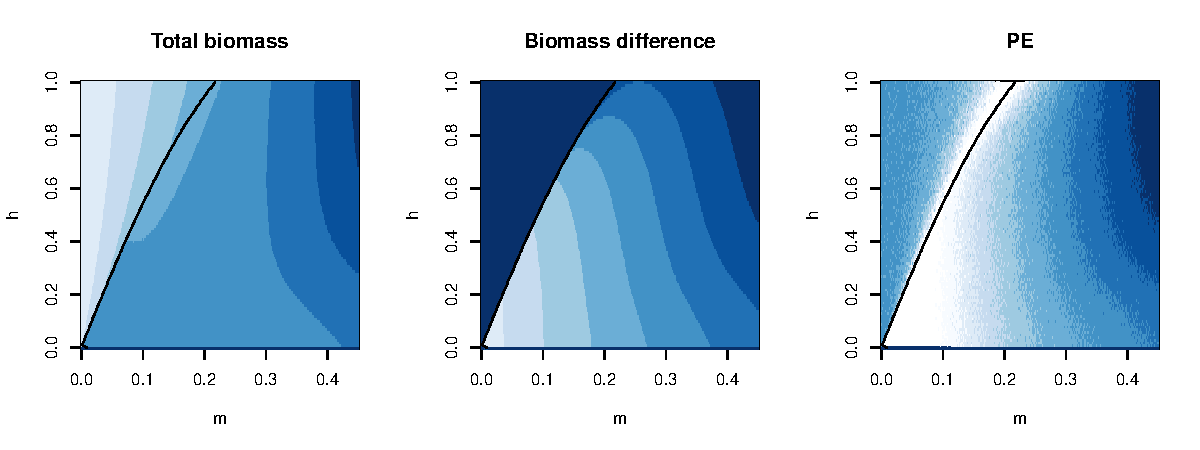
\includegraphics[width=0.8\textwidth]{figs2/fig_MDPE_hm.pdf}
\caption{
(a) Total means $N_t$, (b) difference in means $\Delta N$, and (c) the portfolio effect PE as a function of heritability $h^2$ and a constant stray rate $m$. Light colors = high values.
The black line shows the fold bifurcation separating a single steady state (left) from alternative steady states (right).
(d) The relationship between the time to recovery following a disturbance and the portfolio effect.
} \label{fig:PE}
\end{figure*}

\noindent{\bf (b) Recruitment over a selective landscape}
\noindent Because individuals from the local population are mixed with individuals from the remote population via staying, the resulting trait distribution is a mixed normal with weights corresponding to the proportion of the mixed population that are local individuals, $w_i$, and for the straying individuals, $1-w_i$, where 
\begin{equation}
w_i=\frac{(1-m)N_i(t)}{(1-m) N_i(t) + m N_j(t)}.
\end{equation}
We make two simplifying assumptions.
First, we assume that the distribution resulting from the mix of remote and local individuals, following reproduction, is also normal with a mean value being that of the mixed-normal.
Second, we assume that changes in trait variance through time are minimal, such that $\sigma^2$ is assumed to be constant.



An increasing flow of incoming strays is generally expected to pull the mean trait value of the local population away from its optimum over time, which will decrease its rate of recruitment.
The mean trait value thus changes through time according to the difference equation

\begin{align}
  \label{eq:mu}
  \mu_i(t+1) &= w_i\mu_i(t) + (1-w_i)\mu_j(t) \\ \nonumber
  &+ h^2\sigma^2\frac{\partial}{\partial \mu_i}\ln\left(w_i R_i[\mu_i(t)|\theta_i] + (1-w_i)R_i[\mu_j(t)|\theta_i]  \right),
\end{align}

\noindent where the first two factors determine the mixed normal average of the aggregated local and remote populations.
The partial derivative in the Eq. \ref{eq:mu} determines how the mean trait changes through time due to natural selection \cite{Lande:1976ga}, which is proportional to the change in mean fitness with respect to $\mu_i$.
\\

\noindent {\bf (c) Measuring metapopulation robustness}
\noindent We evaluated metapopulation robustness by measuring the average-CV portfolio effect (PE) \cite{Anderson:2014cx,Schindler:2015gf} as well as the time required for the system to return to a steady state following an induced disturbance to one or both of the populations \cite{Ovaskainen:2002il}.
The average-CV portfolio effect is, as the name implies, the average CV across each population divided by the CV of the aggregate \cite{Anderson:2013gb}, such that


\begin{equation}
\langle{\rm PE}\rangle =\frac{1}{X}\sum_{i=1}^{X} \frac{\sqrt{{\rm VAR}(N_i)}}{{\rm E}(N_i)}\cdot \frac{{\rm E}(N_T)}{\sqrt{{\rm VAR}(N_T)}},
\label{eq:pe}
\end{equation}

\noindent where in this case the number of populations is limited to $X=2$ and the expectations $\rm E(\cdot)$ and variances $\rm VAR(\cdot)$ are evaluated at the steady state.
As the CV of $N_T$ decreases relative to that of the constituent populations, $\langle{\rm PE}\rangle > 1$, and the metapopulation is presumed to become more stable.
{\color{red} A similar measure of metapopulation robustness can be evaluated by measuring the synchronization $\phi$ between populations, where 
\begin{equation}
\label{eq_sync}
\phi = \frac{{\rm VAR}(N_T)}{\left(\sum_{i=1}^N\sqrt{{\rm VAR}(N_i)}\right)^2}.
\end{equation}
By rearranging and substituting eq. (\ref{eq_sync}) into eq. (\ref{eq:pe}), we can observe that $\langle{\rm PE}\rangle \propto \sqrt{\phi}^{-1}$.
Thus, the dynamical diversity of the metapopulation offers a mirror to the portfolio effect, where perfect synchrony ($\phi = 1$) also means $\langle{\rm PE}\rangle = 1$.}
%Moreover, if and only if $\phi \neq 1$, it is expected that as the diversity of the aggregate increases, so should the portfolio effect, and this central thesis is thought to underlie the stability of populations, species, communities and even financial markets.
Portfolio effects greater than unity corresponds to less synchronization ($\phi < 1$) \cite{Loreau:2008ju,Anderson:2014cx,Yeakel:2013vz} and thus a greater potential for demographic rescue among populations, buffering the system as a whole against extinction. 

%Although there are more robust ways to measure the portfolio effect (in particular for comparing the PE across species with different mean-variance relationships; REF: Anderson), its only utlity here is to provide a simple statistical measure of metapopulation persistence.
A more direct way to measure system robustness is to measure the time that it takes the system (measured as the aggregate biomass $N_T$) to recover its steady state abundance following an induced disturbance: systems that recover quickly (shorter recovery times) are more robust than those that recover more slowly (longer recovery times).
Although there is a direct eignvalue relationship between the rate of return following a small pulse perturbation (REF), because we aimed to 1) assess the effects of a large perturbation, and 2) estimate the time required for all transient effects to decay (including dampened oscillations), we used a simulation-based numerical procedure.

Numerically estimating the time that it takes for a perturbed system to relax also permits a more detailed perspective of the potential fragility of the metapopulation.
For example, if populations settle to alternative steady states (alternative steady states in our model requiring one population to be high-density and one low-density), comparing recovery times after a disturbance applied to the high, low, and/or both populations allows for an assessment of which component of the metapopulation has a longer-lasting influence on the system's recovery.
Throughout, we will refer to an increase in the portfolio effects and/or reduction in recovery times as promoting metapopulation robustness, which is expected to have a positive effect on persistence.
\\

\noindent {\bf (d) The effects of density and distance on the rate of straying}
%Density dependent m
\noindent We have so far assumed that the proportion of strays leaving and entering a population is constant, however there is good evidence that at least in some species the straying rate is density dependent \cite{Berdahl:2016dx,Bett:2017ha}.
Specifically, the rate at which individuals stray has been linked directly to a collective decision-making phenomenon, where greater numbers of individuals tend to decrease the rate at which individuals err, reducing the overall proportion of a population that strays.
According to Berdahl et al. \cite{Berdahl:2016dx}, given the probability that an individual strays is $m_0$, the proportion of the local population $N_i(t)$ that strays is

\begin{equation}
  m(t) = m_0\left(1- \frac{N_i(t)}{C+N_i(t)}\right),
  \label{eq:ddm}
\end{equation}

\noindent where $C$ is a half-saturation constant.
We note that at the limit $C\rightarrow \infty$, the density dependent straying rate becomes constant such that $m(t) \rightarrow m_0$, and this corresponds to the original formulation where $m=m_0$.
A similar observation shows that when the population density is very high, $m(t) \rightarrow 0$, and when it is small, individuals operate without regard to collective behavior, meaning $m(t) \rightarrow m_0$.
Thus, for realistic population densities, $m(t) < m_0$.


%Linking m/m0 and thetadiff
The straying rate is intrinsically linked to the distance between the donor and recipient population.
The greater the distance between two populations, the lower the expected rate of straying (REF).
We can account for this interdependence in our model by assuming that $m$ (if the stray rate is constant) or $m_0$ (if the stray rate is density dependent) is a function of the difference between optimal trait values between sites $\theta_i-\theta_j$, which can be assumed to be large if the remote site $j$ is a great distance away from the local site $i$.
If sites $i$ and $j$ are very close, the stray rate is maximized at $m_{\rm max} = 0.5$, assuming both sites are equally attractive to the respective populations.
Thus, we can integrate these two variables by setting $m,m_0 = (1/m_{\rm max} + \epsilon (\theta_i-\theta_j))^{-1}$, where $\epsilon$ sets the sensitivity of a declining $m$ to increasing distance (greater values of $\theta_i-\theta_j$).

\begin{figure*}
  \captionsetup{justification=raggedright,
singlelinecheck=false
}
\centering
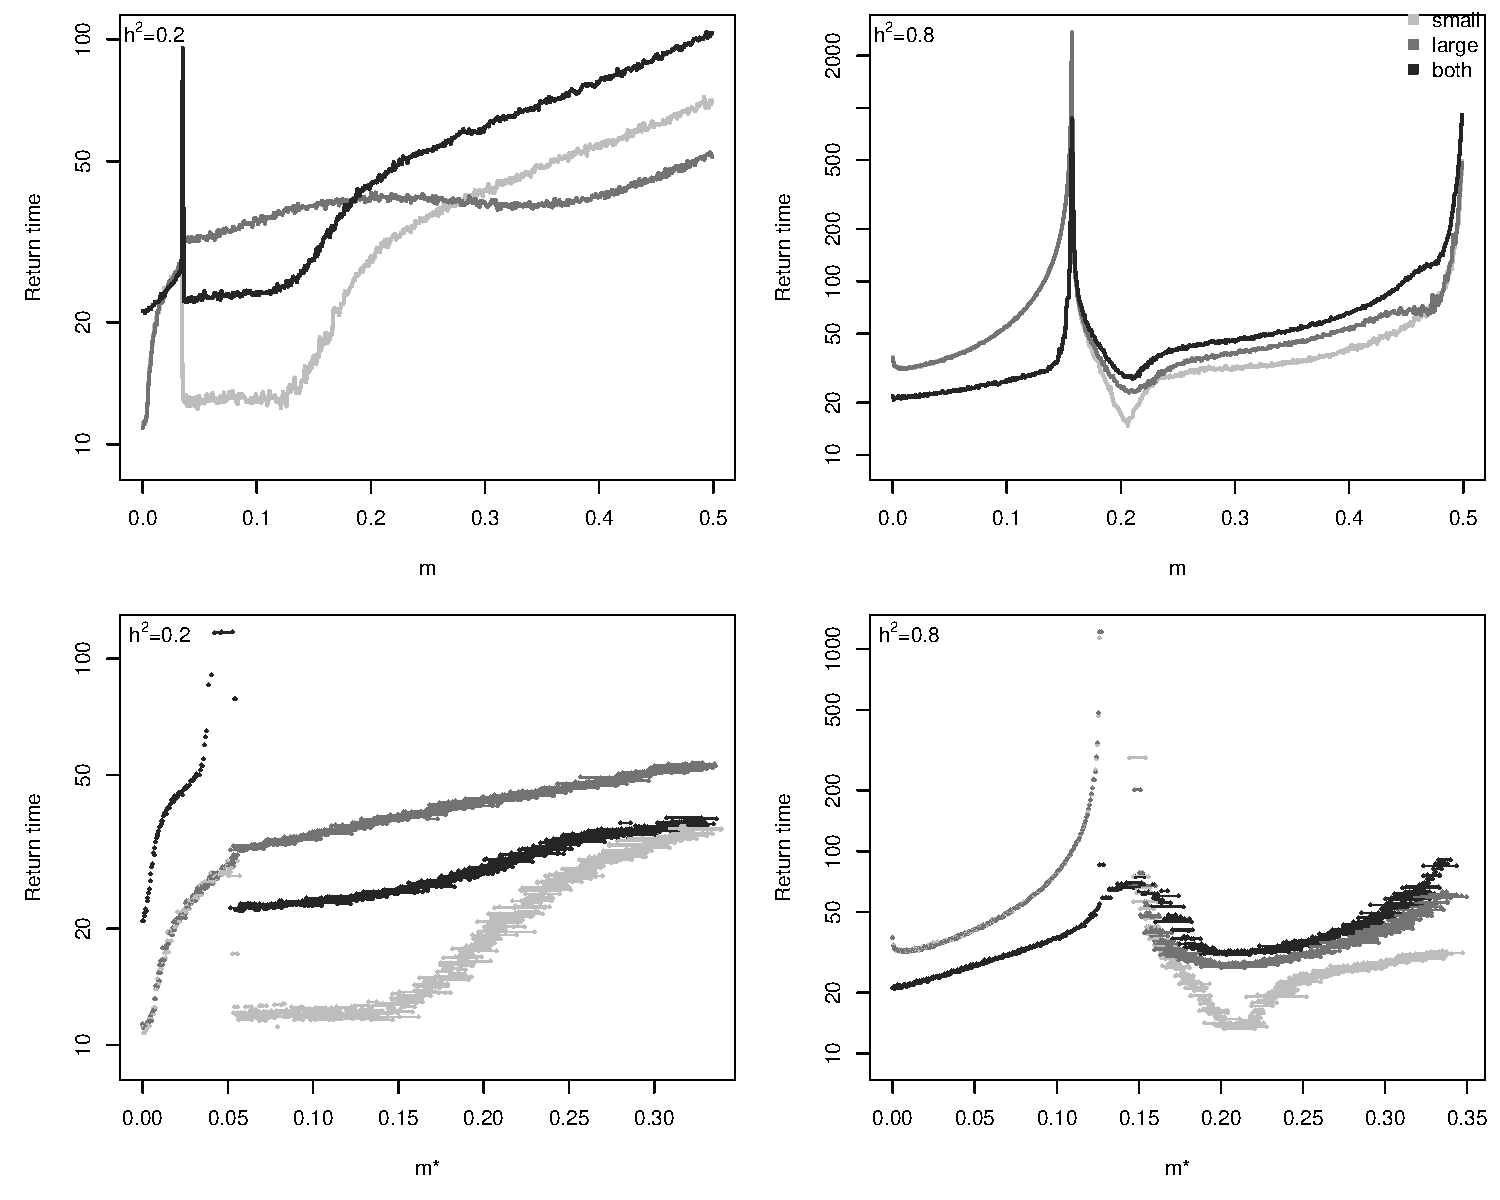
\includegraphics[width=0.9\textwidth]{figs2/fig_relax_comb.pdf}
\caption{
(a, b) Recovery time of $N_T$ following the extinction of either the low-density (light gray) or high-density (gray) population, or the near-collapse of both (dark gray) assuming constant straying rates $m$ and (c, d) density dependent straying rates (evaluated at the steady state $m^*$).
If $m$ is density dependent, in the alternative steady state regime there are two straying rates observed: one each for the low- and high-density populations, respectively, which are linked by a horizontal line.
} \label{fig:relax}
\end{figure*}



\section{Results}

%The effects of trait evolution :: trait heritability, trait variance, and habitat heterogeneity
%% Bifurcation to alternative stable state occurs at higher stray rates with increased trait heritability
%% There is a peak in the portfolio effect directly before this bifurcation is crossed (early warning signal), and then a decline in PE with high m
%% When trait heritability is high, there is a greater sensitivity of total biomass to increasing stray rates, though a LOWER sensitivity of the difference between alternative steady state values for increasing stray rates (and vice versa)
%% For low heritability (h = 0.01 - 0.2 or so), moderate and insensitive changes in total biomass, but large differences between the values of alternative steady states leads to a local maximum for PE at low-moderate stray rates



%Alternative stable states

\noindent{\bf (a) Nonlinear effects of straying on the portfolio effect and recovery time} \\
\noindent Straying generally lowers steady state densities for both populations by \emph{i}) the donor population losing locally-adapted individuals to the recipient population and \emph{ii}) the introduction of maladapted individuals to the recipient population from the donor population, and this accords with observations from natural populations \cite{Bett:2017ha} %, regardless of trait heritability and variance or habitat heterogeneity
The decline in steady state densities is not gradual: as straying increases, the system crosses a fold bifurcation whereby the single steady state for the metapopulation bifurcates into two alternative steady states: one at high biomass, and one at low biomass density (figure \ref{fig:traj}a, \ref{fig:PE}a).
Mean trait values for both populations bifurcate similarly (figure \ref{fig:traj}b), depending on which population attains a low- vs. high-density, which in our system is random due to a small amount of introduced variation in the initial conditions.
The fold bifurcation (the black line in Figs. \ref{fig:PE}a-c) occurs at lower values of the straying rate $m$ with decreased trait heritability $h^2$ (Fig \ref{fig:PE}a,b), indicating that weaker coupling between ecological and evolutionary dynamics in addition to higher rates of straying promotes the appearance of alternative stable states.

Trait heritability has a large impact on the sensitivity of the straying rate to both the aggregate population steady state density ($N^*_T=N^*_1+N^*_2$; figure \ref{fig:PE}a) as well as the difference between steady state densities (the distance between alternative stable states: $\Delta N=|N^*_1-N^*_2|$; figure \ref{fig:PE}b).
Greater trait heritability results in a faster decline in $N_T^*$ with increasing straying rates $m$, but leads to only moderate changes to $\Delta N$.
Conversely, if the trait is less heritable, an increase in the straying rate has little impact on the total biomass density but contrastingly large effects on $\Delta N$.




%Together these changes in steady state population densities in terms of $N_T$ and $\Delta N$ as a function of trait heritability and the rate of straying between populations give rise to highly nonlinear portfolio effects, which we quantify here as

% Nonlinear PE(!!!)

%In the region where there is a single steady state among both populations, we find an low-intermediate portfolio effect ca. ${\rm PE}=1.4$, primarily due to the elevated mean values of $N_T$.
As the fold bifurcation is approached with increasing $m$, the portfolio effect increases sharply due to an amplification in variance within both donor and recipient populations ${\rm VAR}(N_{i,j})$.
This variance increase is the product of a dynamical process known as critical slowing down that occurs near fold bifurcations \cite{Scheffer:2009gg}, a phenomenon that some have suggested may serve as an early warning indicator for approaching phase transitions \cite{Scheffer:2009gg,Lade:2012eu,Anonymous:2013br,Dakos:2014br}.
For larger values of $m$ (to the right of the fold bifurcation in Fig \ref{fig:PE}a-c), where alternative steady states occur, the portfolio effect declines steadily as the CV of $N_T$ increases.
The decline over $m$ is more gradual if trait heritability is low, and steeper if trait heritability is high (figure \ref{fig:PE}c).



% \noindent{\bf (c) Rates of recovery following catastrophic collapse}\\ 
% Return time as a measure of system persistence and relation to PE
As the portfolio effect is highly sensitive to the rate of straying between populations, so is the time required for the system to recover to a steady state following a large disturbance.
We measured the time required for the system $N_T$ to relax to its steady state following three types of induced disturbance: (\emph{i}) extinction of the low-density population; (\emph{ii}) extinction of the high-density population (scenarios \emph{i} and \emph{ii} are equivalent if the system is in the single steady state regime); (\emph{iii}) near-collapse of both populations where just 1.0\% of each survives.
In general, we find that the average-CV portfolio effect is negatively correlated with recovery time (figure \ref{fig:PE}d), indicating that for our system both measures are valuable indicators of metapopulation robustness.
Because we can assess the time to recovery in response to the various disturbance types described above, this allows us to gain an in-depth perspective into the fragility of the metapopulation as a function of straying rate.

At low rates of straying both populations are subject to the same steady state, such that extinction of either population results in the same recovery time, and when trait heritability is low, the time required to recover following the extinction of either population is generally less than or equal to the recovery time after near-collapse of both (figure \ref{fig:relax}a).
In the alternative stable state regime where straying rates are higher, extinction of the smaller population results in the shortest recovery time, whereas as $m$ increases, extinction of the larger population results in the shortest recovery time.
Because the mean trait values of both populations are skewed towards those of the high-density site, when the low-density population collapses under high rates of straying, selection against the flood of maladapted individuals that stray into the recovering extends the length of time required for it to return to its steady state (figure \ref{fig:relaxtraj_ldlh}).
Alternatively, when the high-density population collapses under high straying rates, the low-density population suffers loss as well due to the absence of incoming strays such that both populations must recover (figure \ref{fig:relaxtraj_hdlh}).

Increased trait heritability flips this relationship by increasing the response of trait evolution to changes in demography (figure \ref{fig:relax}b).
When straying rates are low, metapopulations that suffer near-collapse of both populations recover more quickly than systems suffering extinctions of either population.
When straying rates are higher such that the system is in the alternative stable state regime, the metapopulation always recovers more quickly if the small population is lost (figure \ref{fig:relaxtraj_ldhh}), whereas the time to recovery is maximized if both populations suffer near-collapse.
When the high-density population goes extinct, the stronger response of selection permits the surviving low-density population to grow quickly and fill the high-density state (figure \ref{fig:relaxtraj_hdhh}).
Near the onset of the fold bifurcation, recovery times increase explosively regardless of straying rate, heritability, or disturbance type.
%For straying rates in the alternative steady state regime, extinction of the smaller population consistently results in the shortest time to recovery.


\begin{figure}
  \captionsetup{justification=raggedright,
singlelinecheck=false
}
\centering
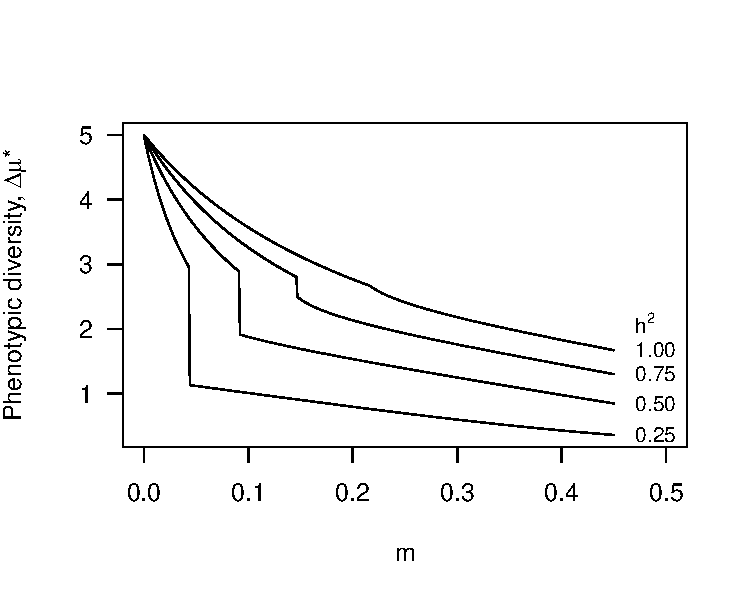
\includegraphics[width=0.5\textwidth]{figs2/fig_traitdiff.pdf}
\caption{
Phenotypic diversity ($\Delta \mu^*$) evaluated at the steady state as a function of straying rate $m$ and trait heritability $h^2$. The descrete jump occurs as the system crosses the fold bifurcation; lower phenoytic diversity emerges with higher straying rates and in the alternative steady state regime. 
} \label{fig:traitdiff}
\end{figure}

%Lowering Phenotypic diversity with increasing straying rate
Increased rates of straying lowers phenotypic diversity ($\Delta \mu^* = |\mu_i(t)-\mu_j(t)|$, evaluated at the steady state) because both local and remote populations are increasingly homogenized.
The loss of phenotypic diversity with increased straying is greater if trait heritability is low because the selective forces acting against trait means far from the local optima are lessened. % with decreased $h^2$.
Less intuitively, we observe a discrete jump towards low phenotypic diversity as the fold bifurcation is crossed (figure \ref{fig:traitdiff}).
Although the development of alternative stable states elevates the portfolio effect due to the variance-dampening effects of the aggregate, entering this dynamic regime also results in a substantial decline in phenotypic diversity, which may have less predictable adverse effects on the population. 
\\

\begin{figure}
  \captionsetup{justification=raggedright,
singlelinecheck=false
}
\centering
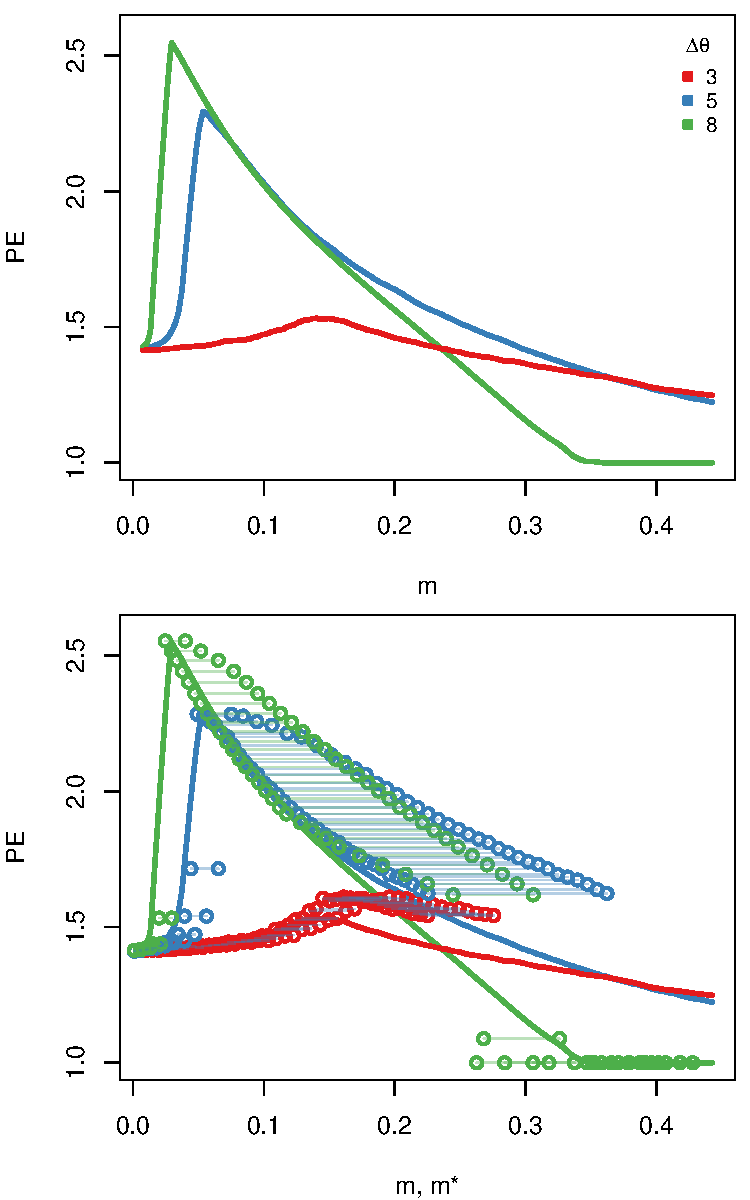
\includegraphics[width=0.4\textwidth]{figs2/fig_thetaPEmvm.pdf}
\caption{
(a) Median portfolio effect as a function of stray rate $m$ given heritability is $h^2 < 0.5$ for habitats with increasing heterogeneity as measured by the difference in regional trait optima $\Delta \theta$.
(b) Median portfolio effects as shown in (a) are denoted by the solid lines. 
Point pairs connected by a horizontal line represent the PE as a function of density dependent straying rates, evaluated for both low- and high-density populations at equilibrium. The lower straying rate of a pair is for the larger population; the higher straying rate is for the smaller population.
The different steady state regimes that give rise to the range of straying rates were obtained by varying the individual straying probability $m_0$ (where $m_0$ and $m^*$ are linearly related).
} \label{fig:thetaPE}
\end{figure}

%% Increased habitat heterogeneity
  %%% 1) exaggerates lowering of mean biomass with increasing stray rates
  %%% 2) increases the likelihood of alternative stable sites & increases the differences in alternative stable state values with increasing stray rates
  %%% 3) decreases the PE (!!)

\noindent{\bf (b) The influence of habitat heterogeneity on metapopulation robustness}\\ 
\noindent Increasing differences in optimal trait values between sites ($\Delta\theta = \left|\theta_i - \theta_j\right|$) corresponds to greater regional differences in the conditions that favor alternative trait complexes, which we interpret here as greater habitat heterogeneity.
Although trait heritability among salmonids is variable, most life history traits show $h^2 <0.5$ \cite{Carlson:2008hl}, and we largely focus additional analyses on that range.
If both populations are isolated, natural selection will direct the mean trait values of both populations towards their respective optima, such that $\mu_i(t) \rightarrow \theta_i$ as $t\rightarrow\infty$.
%difference in optimal trait values between the local and remote populations, which we call .
With the onset of straying, we find that increasingly divergent trait optima generally lower $N_T$ and exaggerate $\Delta N$ (figure \ref{fig:thetadiffN}), such that the biomass distribution becomes increasingly uneven. %I've checked this - it's a theshold type (logistic) response Supp fig?
The impact of habitat heterogeneity on the portfolio effect and recovery time is more complex, serving to emphasize the nonlinear relationship between rates of straying and metapopulation robustness. %regardless of heritability.
%The rate of straying that gives rise to a large PE at the fold bifurcation is conditioned on the difference in optimal trait values between the local and remote populations, which we call $\Delta\theta = \sqrt{(\theta_i - \theta_j)^2}$.
As habitat heterogeneity increases, alternative stable states appear for lower straying rates -- with the crossing of the fold bifurcation, accompanied by a peak in the PE -- whereas the magnitude of increase in the PE increases (figure \ref{fig:thetaPE}a), reducing recovery time (figure \ref{fig:relaxtheta}).
For increased rates of straying, greater habitat heterogeneity erodes the PE and increases the recovery time (figure \ref{fig:thetaPE}a, figure \ref{fig:relaxtheta})
Taken together, habitat heterogeneity, as measured as the differences in trait optima between two habitats, promotes robustness when straying rates are low, but erodes robustness when straying rates are high.
%This means that alternative stable states can emerge with relatively little dispersal between sites (figure \ref{fig:thetaPE}), however the increased PE (and shorter recovery times).
\\




% Density dependent m
%% Because m[t] @ steady state 0<m[t]<m0, we observe the same dynamics for higher m0 as we do for lower constant m.
%% Higher rates of straying are tolerable (there is a not a decline in PE for very high m0 as there is for constant m)

\noindent{\bf (c) The effects of density dependent straying}\\
\noindent If we assume that the rate of straying is density dependent, the probability that an individual strays $m_0$ determines the rate of straying within the population, such that $m(t)$ becomes lower as $N(t)$ increases due to the effects of collective decision-making \cite{Berdahl:2016dx} (Eq. \ref{eq:ddm}).
%Because our analyses concern steady state conditions, the inclusion of density-dependent straying does not have a large impact on the qualitative nature of our findings (figure \ref{fig:ddm}).
Density dependence alters the straying rate at steady state population densities because $0 < m^* < m_0$, and this serves to rescale both the strength of the PE as well as the recovery time, but importantly does not change the qualitative nature of our findings for constant straying rates.
In the alternative stable state regime, because the each population exists at different steady state densities, there are likewise two alternative straying rates $(m_i^*,m_j^*)$: the higher straying rate is associated with the low-density population, and the lower straying rate is associated with the high-density population.
We assessed metapopulation robustness across a range of $(m_i^*,m_j^*)$ values by varying $m_0$, which is positively and linearly related to $(m_i^*,m_j^*)$.

%Recovery times
The recovery times for systems with constant and density dependent straying both show similar trends for a given $m$ and $m^*$ (figure \ref{fig:relax}c,d), however there are some distinct quantitative differences.
When the straying rate and trait heritability are low, near-collapse of both populations result in longer than expected recovery times, whereas in the alternative stable state regime (higher $m^*$), the recovery times for different disturbance types are very similar to systems with a constant $m$ (figure \ref{fig:relax}c; note difference in x-axis scales).
There is greater similarity in the recovery times for constant and density dependent $m$ systems when trait heritability is high.

As with recovery time, we find that the portfolio effects generated in systems with density dependent straying are qualitatively similar to systems with constant straying, however there are some important quantitative differences.
First, the PE associated with the high-density (low $m^*$) population is the same as that for a system with a constant $m$ (figure \ref{fig:thetaPE}b).
As such, the difference in $m^*$ among low- and high-density populations appears to matter less than the straying generated by the high-density population.
However, as $m^*$ increases, we observe a higher PE than that generated by systems with constant $m$.
This higher PE at increased $m^*$ is mirrors recovery times that are also lower than those observed for systems with constant $m$ (figure \ref{fig:relax}).
Together this suggests that although density-dependent straying does not appear to change the `dynamic landscape' in our minimal model, we do find evidence that it can promote robustness, particularly when populations are low and straying is correspondingly high.
% 
% 
% In a metapopulation with density dependent straying, the lower straying rate of the high-density population generates a portfolio effect that would be expected if straying were constant.
% 
% A metapopulation with density dependent straying has a portfolio effect 
% 
% equal to that of a metapopulation with constant straying
% 
% as would be expected for a metapopulation with a constant straying rate equalt to that of the 
% 
% We find that the by-definition lower straying rate of the high-density population (left-most of the paired points in figure \ref{fig:thetaPE}b) largely determines the portfolio effect for the metapopulation.
% In other words, 
\\

\begin{figure*}
  \captionsetup{justification=raggedright,
singlelinecheck=false
}
  \centering
  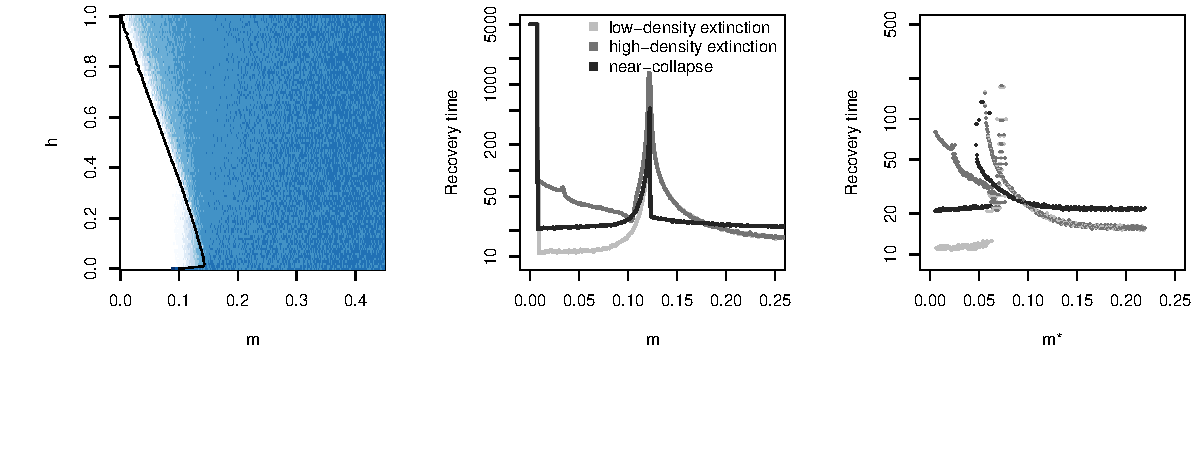
\includegraphics[width=0.8\textwidth]{figs2/fig_MDPE_hm_mtheta_rt.pdf}
  \caption{
  Assuming that the rate of straying is linked directly to habitat heterogeneity. A low stray rate corresponds to very different (or distant) habitats (high $\Delta\theta$), whereas a higher rate of straying corresponds to very similar (or nearby) habitats (low $\Delta\theta$).
  (a) Portfolio effect over constant straying rate $m$ and trait heritability $h^2$.
  (b-c) Recovery times for three disturbance types for (b) constant $m$ and (c) density dependent straying rate at the steady state $m^*$.
  } \label{fig:mtheta}
\end{figure*}


% When m and thetadiff are linked
%%Constant m
  %%% Low stray rate (high theta1-theta2) leads to alternative stable states and relatively low PE ~ sharp transition
  %%% High stray rate (low theta1-theta2) increases the steady state (and no A.S.S.)... 
  %%% This suggests that space naturally buffers against the negative effects of mixing dissimilar populations, however it is NOT SMOOTH
  %%% This is particularly true for low heritability. High heritability eliminates the A.S.S. region
  %%% (!!!) Even low levels of straying from distant populations can result in highly divergent alternative steady states! THIS IS A COOL RESULT

\noindent{\bf (d) Distance dependent straying and habitat heterogeneity}\\ 
\noindent We have so far treated $\Delta\theta$ and $m$ as independent parameters, however we may also assume that if environmental heterogeneity increases with distance, the rate of straying may be expected to decline given that individuals will stray less into distant habitats. %-- in particular North-South difference if trait optimality is largely temperature-dependent --
If we incorporate this interdependence of $m$ and $\Delta\theta$, low rates of straying correspond to mixing dissimilar (distant) populations, and high rates of straying would correspond to mixing similar (nearby) populations.

We find that alternative stable states now appear at low straying rates, which corresponds to greater $\Delta\theta$.
As the straying rate increases, a single stable state emerges.
As before, the portfolio effect is higher in the alternative stable state regime, with a sharp decline in the PE as the straying rate becomes larger (figure \ref{fig:mtheta}a).
This is in accordance with intuition as increasing straying rates mean that two very similar populations are mixing, such that the strength of selection on recruitment is lessened.

This dynamic is more complex when we observe the recovery times for systems with either a constant (figure \ref{fig:mtheta}b) or density dependent (figure \ref{fig:mtheta}c) straying rate.
Although recovery times are lowest in the alternatice stable state regime ($m<0.1$), this is only true if the low-density population suffers extinction.
Alternatively, at low rates of straying between dissimilar (distant) populations, recovery times become maximized if the high-density population suffers extinction.
As rates of straying -- and the similarity of trait optima -- increase, extinction of either population requires less time for recovery than near-collapse of both.




% That alternative stable states appear and that PE becomes severely depressed for very low rates of straying is surprising: this means that even a small amount of mixing of populations from distant or dissimilar populations can qualitatively alter the dynamics of the metapopulation, regardless of trait heritability.
%(for the discussion: an example of this situation may be the salmon populations during the last glacial maximum, where any mixing would be from geographically distant populations)



\section{Discussion}

We have shown that dispersal between populations, coupled with localized selection against donor phenotypes, has a large and nonlinear impact on dynamic properties that directly impacts metapopulation robustness, and by extension persistence.
Although there are various ways to measure `robustness' (REF:TREE), we employ two measures: 
1) the average-CV portfolio effect, a statistical metric commonly used to assess the fragility of salmon populations; 
2) the recovery time, defined here as the time required for the aggregate metapopulation biomass $N_T$ to return to its steady state after different types of induced disturbances, which is mechanistically linked to the likelihood of persistence (REF).
In our minimal model of dispersal and natural selection between two populations, we show that these phenomenological and mechanistic descriptors of metapopulation robustness are tightly coupled (figure \ref{fig:PE}d).

%Alternative steady states & critical slowing
The immigration of dispersing strays with trait values far from the local optimum generally lowers the combined steady state biomass $N_T$ and increases the likelihood that the system gives way to alternative steady states, pushing one of the populations close to extinction.
The formation of alternative stable states in our system is a relatively common example of spatial pattern formation, and occurs above a threshold straying rate.
Pattern formation can occur as a consequence of myriad ecological processes, including habitat selection (REFS), aggregation of individuals (REFS), local environmental conditions (REFS), or interspecific interactions like competition (REFS). 
It is also well known to occur with the onset of spatially or diffusion-induced instabilities (Turing instabilities, REFS). 
Here, we describe an interesting alternative mechanism through which pattern formation in local densities can occur, when the onset of movement mediated maladaptation leads to local differences in reproductive rates that yield differences in densities that would, in the absence of straying, be the same. 
This mechanism of pattern formation through the simultaneous interplay between ecological and evolutionary dynamics may open up new areas of research.


To what extent the existence of alternative stable states promotes or diminishes the system as a whole is a matter of perspective.
On the one hand, one population is pushed to a low-density state (figure \ref{fig:traj}) with a lower total biomass of the aggregate (figure ]ref{fig:PE}a), suggesting that the system is more fragile.
On the other hand, the presence of \emph{just enough} straying to cause formation of alternative stable states both increases the portfolio effect (figure \ref{fig:PE}c) and reduces the rate of return -- particularly if straying is density dependent (figure \ref{fig:relax}c,d) as might be common in systems with collective navigation (REF).

%The bifurcation and critical slowing down
Although the portfolio effect is negatively correlated with recovery time, there is one exception: the point of transition from a single steady state to alternative steady states, which occurs at the fold bifurcation (REF).
At this point, the portfolio effect is maximized, but so is the recovery time (figures \ref{fig:PE}, \ref{fig:relax}).
This suggests that while the sharply increasing variance of the individual populations is dampened by aggregation, a large disturbance will have a much greater adverse effect due to exponentially longer recovery times.
Whether the change in variance, also known as critical slowing down, as the alternative steady state regime is approached could be used as an early warning signal of an oncoming phase transition is a hotly debated topic (REFS).
The detectability of such changes in dynamical behavior among salmonids appears to be idiosyncratic across species, though the difficulty in measuring critical slowing down may - ironically - be masked by large portfolio effects \cite{Krkosek:2014ch}.

%Comparing recovery times
Previous theoretical work has shown that the largest perturbations lead to the longest recovery times \cite{Ovaskainen:2002il}.
In terms of relative biomass lost, the largest perturbation that we investigate is the near-collapse of both fisheries, where only 1\% of the preperturbation population densities survive, however whether this disturbance results in the longest recovery time depends largely on the rate of straying and trait heritability.
For example, when straying and trait heritability are low (figure \ref{fig:relax}a,c) the extinction of the larger population maximizes return time, whereas if straying is high, near-collapse maximizes return time.
The latter is always true in the alternative stable state regime is trait heritability is high (figure \ref{fig:relax}b,d)


%Density dependent straying
This issue is largely focused on the notion that straying in biological systems where movement is a function of collective navigation may be density dependent.
Berdahl et al. (REF) provided a mechanistic theory for density dependent straying where the proportion of the population that strays is less than the probability that a single individual (as illustrated by \emph{Kevin}; figure \ref{fig:xkcd}) takes the wrong turn.
Neither the transient nor asymptotic dynamics that we describe here qualitatively differ as a function of whether the rate of straying is constant or density dependent, however we observe important quantitative differences that suggest density dependent straying may play an important role in the persistence of metapopulations over evolutionary time.

First, density dependent straying reduces the time to recovery following an induced disturbance, and this is particularly true if (\emph{i}) trait heritability is low, and (\emph{ii}) in the case of near-collapse of both populations (figure \ref{fig:relax}c).
This dynamic emerges because although both populations are near-collapse, the mean trait values of both are scewed towards those of the high-density population.
As the low-density population has also collapsed, and the mean trait values of the system favor the high-density population, it grows more quickly, recovering faster (figure \ref{fig:relaxtraj_bothlh}).
Second, density dependent straying increases the effective portfolio effects when the steady state straying rate is higher (for both low- and high-density populations).
Third, while habitat heterogeneity is interpreted here in elevating the difference in trait optima between sites, it both increases the portfolio effect and lowers recovery time at low rates of straying, but has the opposite effect at higher rates of straying.
Surprisingly, we find that density dependent straying both exaggerates the negative effects when $m^*$ is low (marginally lower portfolio effects, but subsatially longer return times; figures \ref{fig:thetaPE}b, \ref{fig:relaxtheta}a,b) and exaggerates the positive effects when $m^*$ is high (higher portfolio effects, abd shorter return times). 

HAVENT EDITED FURTHER

Trait heritability determines the coupling between ecological and evolutionary dynamics, effectively setting the strength of natural selection.
Among salmon species, recruitment among local populations is highly sensitive to local climatic conditions, with temperature thought to play a central role (REFS).
Populations distributed across a temperature gradient are assumed to be locally adapted to different temperature regimes, such that migration between them should take into account differential environmental effects on the recruitment of mixed populations.
\citeauthor{Carlson:2008hl} showed heritability 0.1-0.3.
Our results show that trait heritability has large effects on both metapopulation persistance as well as phenotypic diversity, particularly in the regime of low-to-moderate straying rates.




%Coupling distance: North-South vs East-West







\bibliography{aa_kevin}


\beginsupplement


\begin{figure}
  \captionsetup{justification=raggedright,
singlelinecheck=false
}
\centering
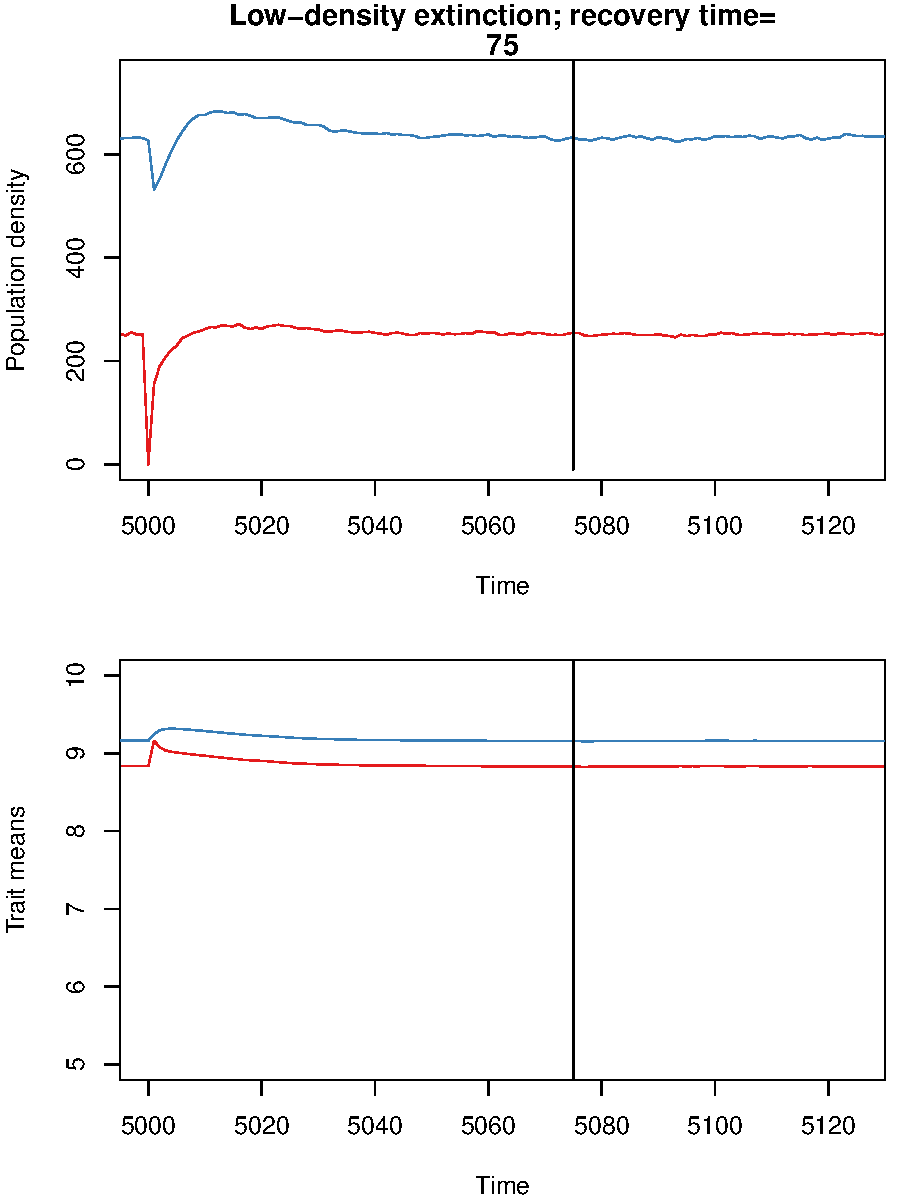
\includegraphics[width=0.35\textwidth]{figs2/fig_relax_small.pdf}
\caption{
Extinction of low-density population with a high constant straying rate $m=0.4$ and low trait heritability $h^2=0.2$ (see figure \ref{fig:relax}a).
Black line marks the calculated point of recovery post-perturbation.
Trait optima are $\theta_1 = 10$ (blue population trajectory) and $\theta_2 = 5$ (red population).
} \label{fig:relaxtraj_ldlh}
\end{figure}

\begin{figure}
  \captionsetup{justification=raggedright,
singlelinecheck=false
}
\centering
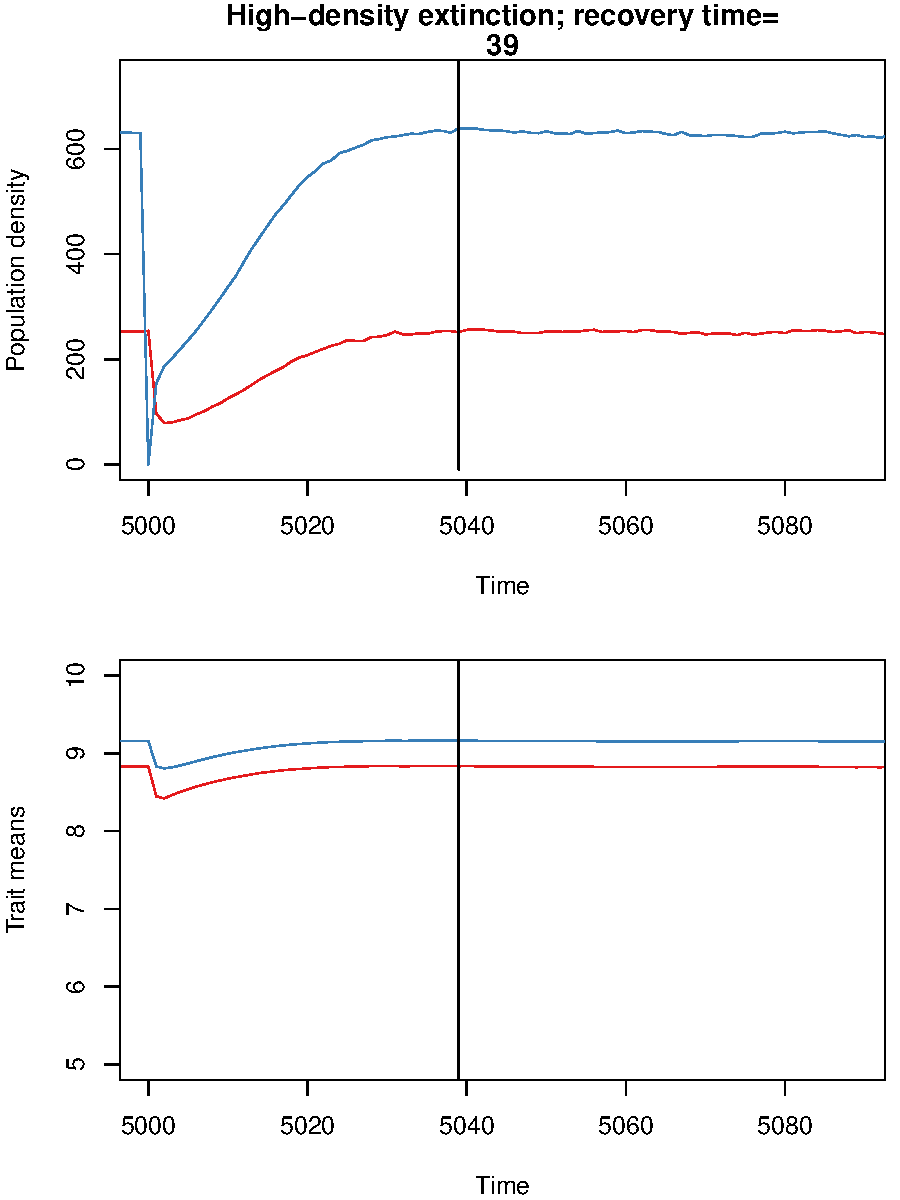
\includegraphics[width=0.35\textwidth]{figs2/fig_relax_large.pdf}
\caption{
Extinction of high-density population with a high straying rate $m=0.4$ and low trait heritability $h^2=0.2$ (see figure \ref{fig:relax}a).
Black line marks the calculated point of recovery post-perturbation.
Trait optima are $\theta_1 = 10$ (blue population trajectory) and $\theta_2 = 5$ (red population).
} \label{fig:relaxtraj_hdlh}
\end{figure}

\begin{figure}
  \captionsetup{justification=raggedright,
singlelinecheck=false
}
\centering
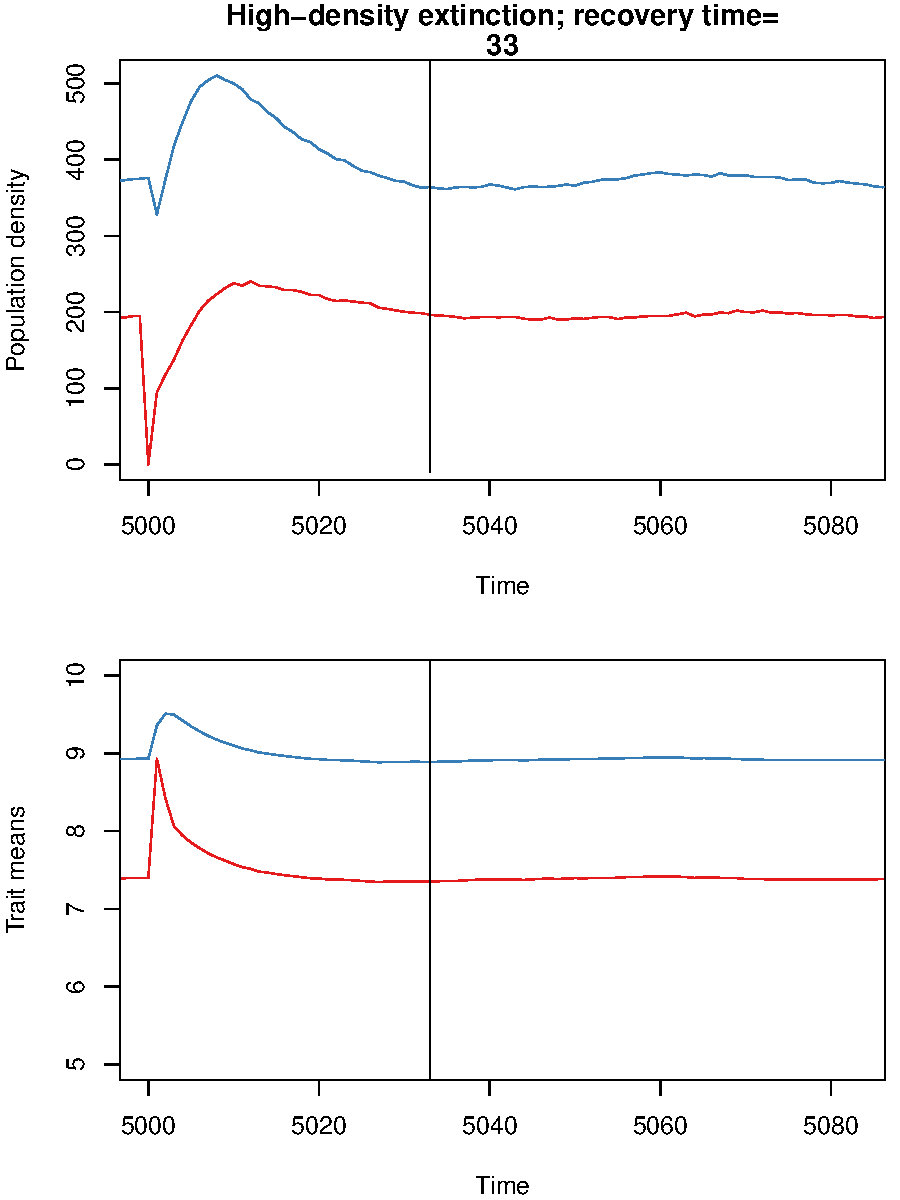
\includegraphics[width=0.35\textwidth]{figs2/fig_relax_small_highh.pdf}
\caption{
Extinction of low-density population with a high constant straying rate $m=0.4$ and high trait heritability $h^2=0.8$ (see figure \ref{fig:relax}a).
Black line marks the calculated point of recovery post-perturbation.
Trait optima are $\theta_1 = 10$ (blue population trajectory) and $\theta_2 = 5$ (red population).
} \label{fig:relaxtraj_ldhh}
\end{figure}

\begin{figure}
  \captionsetup{justification=raggedright,
singlelinecheck=false
}
\centering
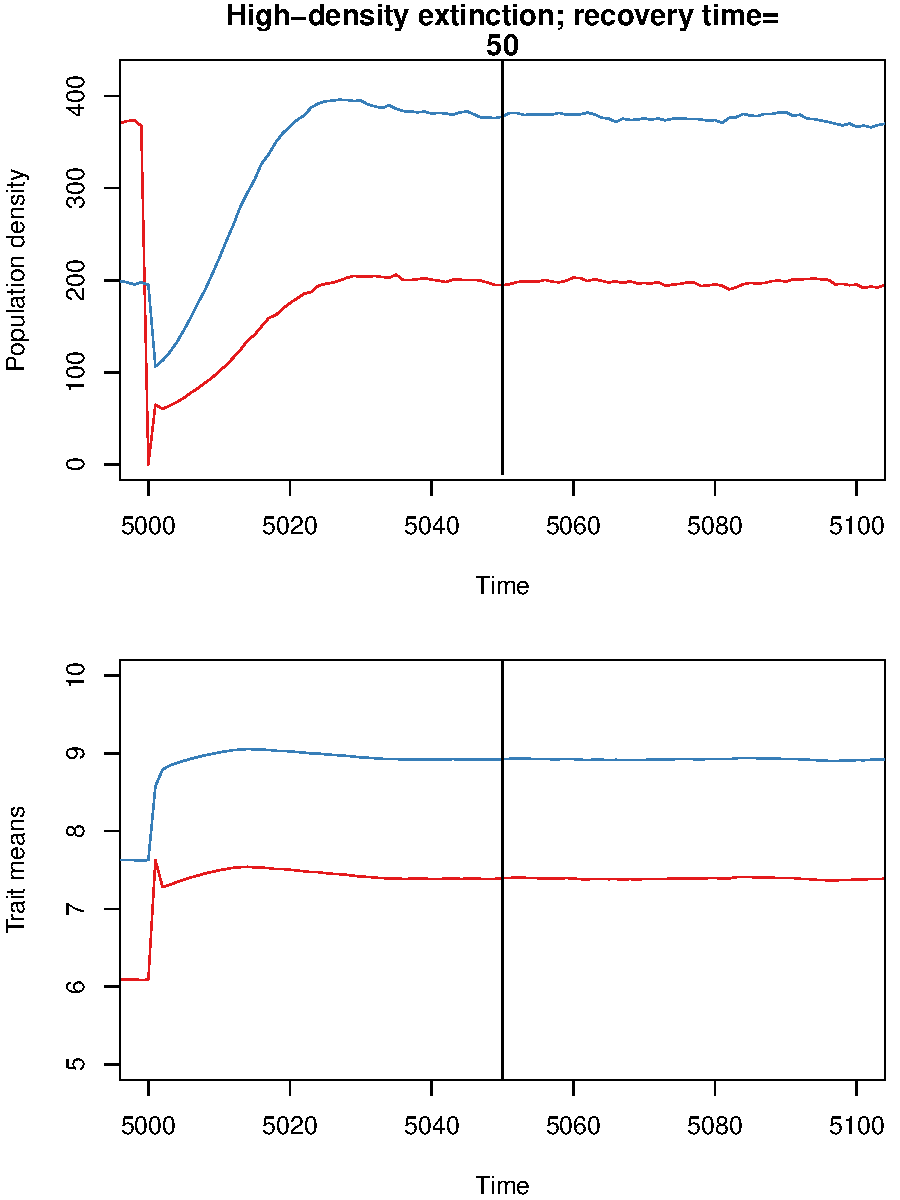
\includegraphics[width=0.35\textwidth]{figs2/fig_relax_large_highh.pdf}
\caption{
Extinction of high-density population with a high straying rate $m=0.4$ and high trait heritability $h^2=0.8$ (see figure \ref{fig:relax}a).
Black line marks the calculated point of recovery post-perturbation.
Trait optima are $\theta_1 = 10$ (blue population trajectory) and $\theta_2 = 5$ (red population).
} \label{fig:relaxtraj_hdhh}
\end{figure}



\begin{figure}
  \captionsetup{justification=raggedright,
singlelinecheck=false
}
\centering
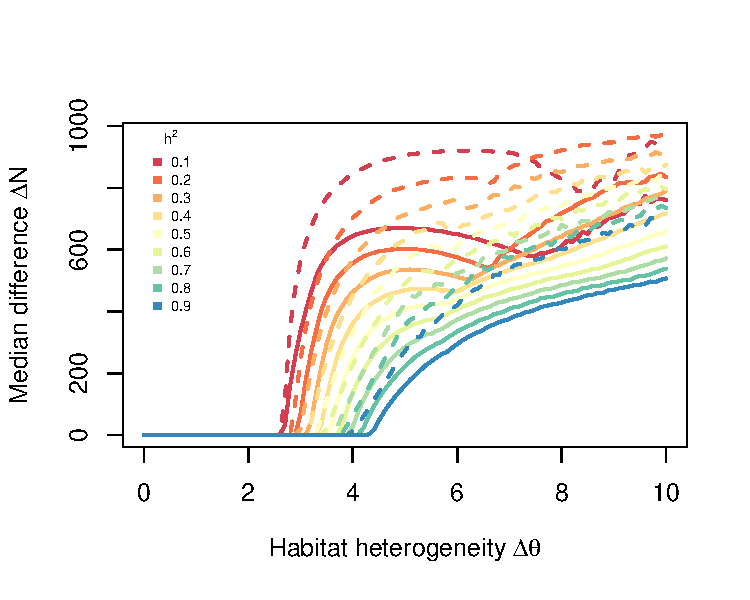
\includegraphics[width=0.35\textwidth]{figs2/fig_thetadiffN.pdf}
\caption{
Median difference in population densities taken over the straying rate as a function of habitat heterogeneity $\Delta\theta$.
Solid lines are for constant $m$; dashed lines are for density dependent $m$} \label{fig:thetadiffN}
\end{figure}



\begin{figure}
  \captionsetup{justification=raggedright,
singlelinecheck=false
}
\centering
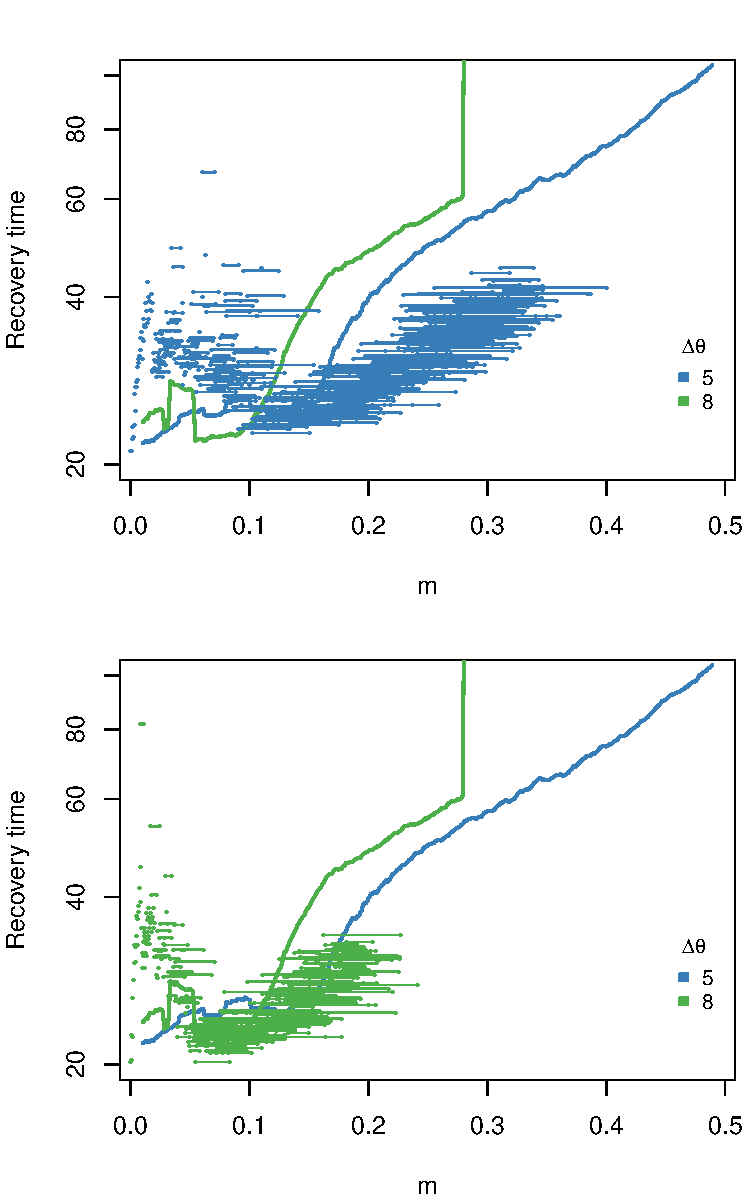
\includegraphics[width=0.35\textwidth]{figs2/fig_relaxtheta.pdf}
\caption{
Recovery time as a function of straying rate $m$ and habitat heterogeneity $\Delta\theta$.
} \label{fig:relaxtheta}
\end{figure}

\begin{figure}
  \captionsetup{justification=raggedright,
singlelinecheck=false
}
\centering
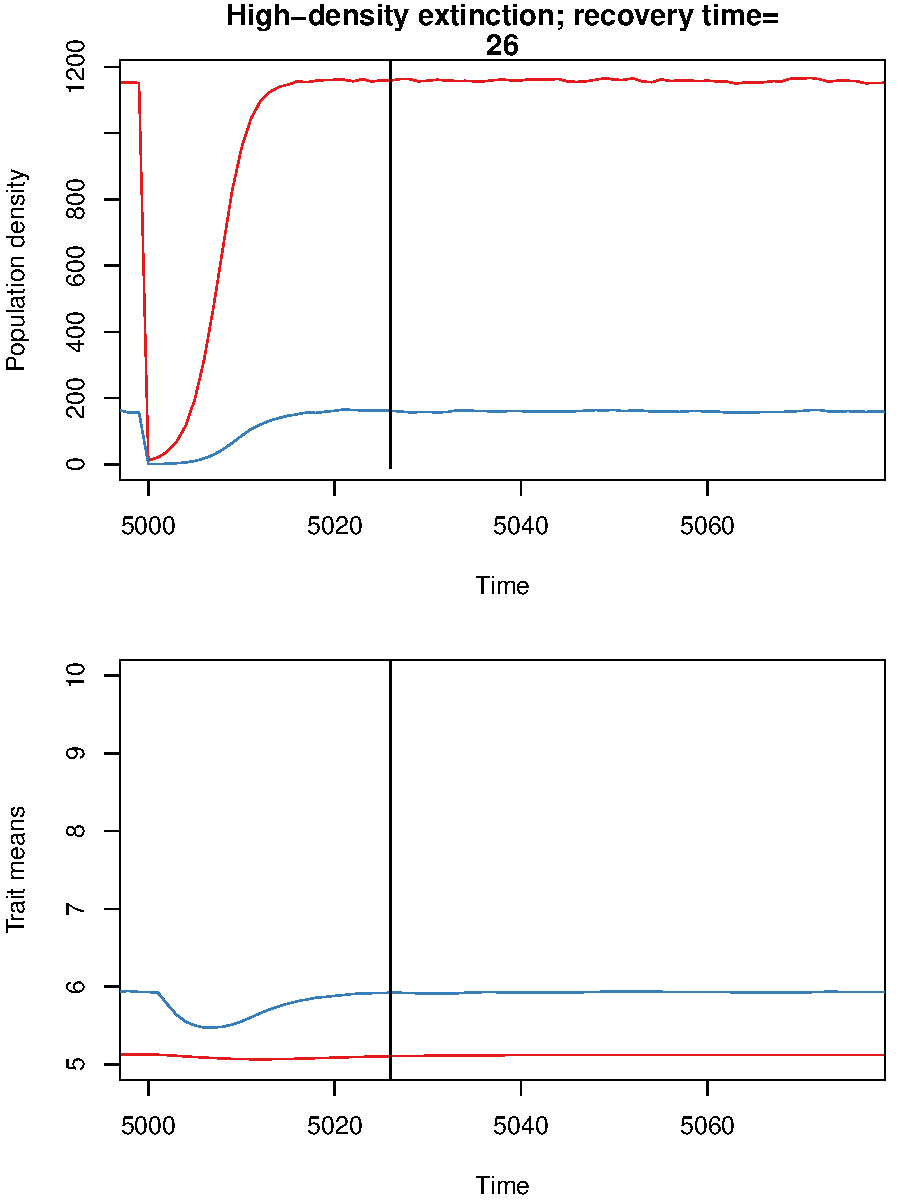
\includegraphics[width=0.35\textwidth]{figs2/fig_relax_both_lowh.pdf}
\caption{
Near collapse of both populations with a low straying rate $m=0.1$ and low trait heritability $h^2=0.2$ (see figure \ref{fig:relax}a).
Black line marks the calculated point of recovery post-perturbation.
Trait optima are $\theta_1 = 10$ (blue population trajectory) and $\theta_2 = 5$ (red population).
} \label{fig:relaxtraj_bothlh}
\end{figure}




% \begin{figure*}[h!]
%   \captionsetup{justification=raggedright,
% singlelinecheck=false
% }
% \centering
% \begin{subfigure}[t]{0.55\textwidth}
% \centering
% 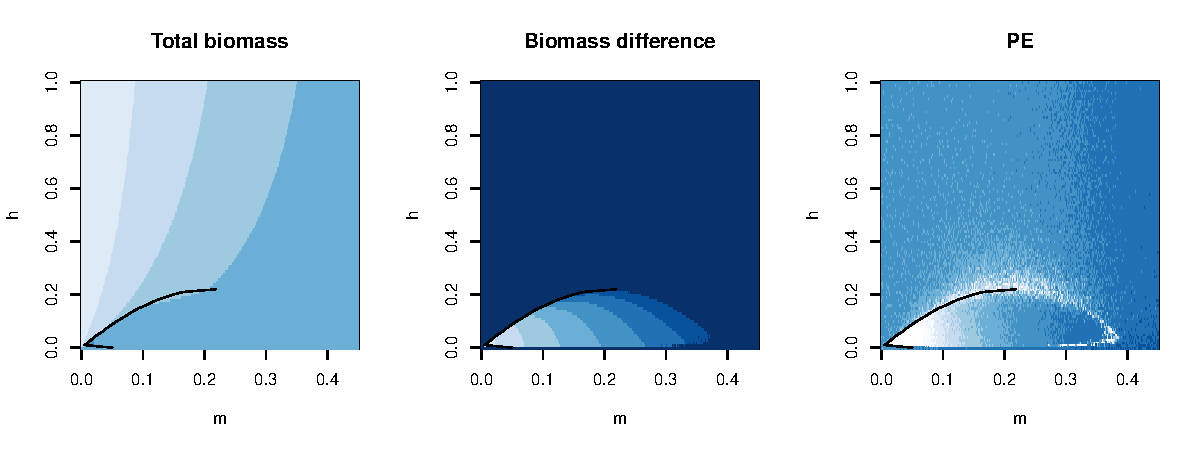
\includegraphics[width=\textwidth]{figs2/fig_MDPE_hm_theta3.pdf} 
% \caption{Low habitat heterogeneity ($\Delta\theta=3$)} \label{fig:thetadiff1}
% \end{subfigure}
% \begin{subfigure}[t]{0.55\textwidth}
% \centering
% 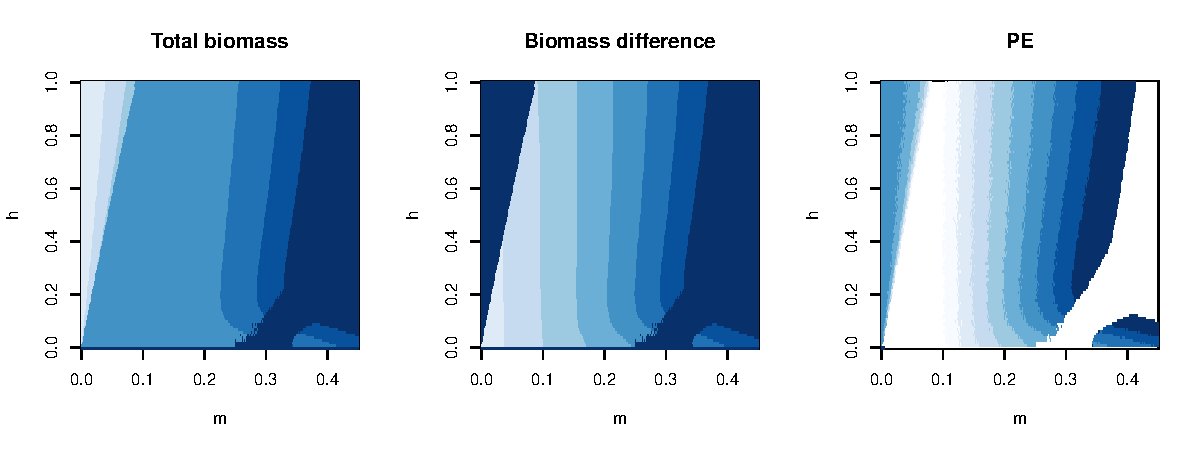
\includegraphics[width=\textwidth]{figs2/fig_MDPE_hm_theta8.pdf} 
% \caption{High habitat heterogeneity ($\Delta\theta=8$)} \label{fig:thetadiff2}
% \end{subfigure}
% \caption{Total means $N_t$, difference in means $\Delta N$, and the portfolio effect PE for different habitat heterogeneities $\Delta\theta$. Light colors = high values.
% }
% \end{figure*}


% \begin{figure*}[h!]
%   \captionsetup{justification=raggedright,
% singlelinecheck=false
% }
% \centering
% 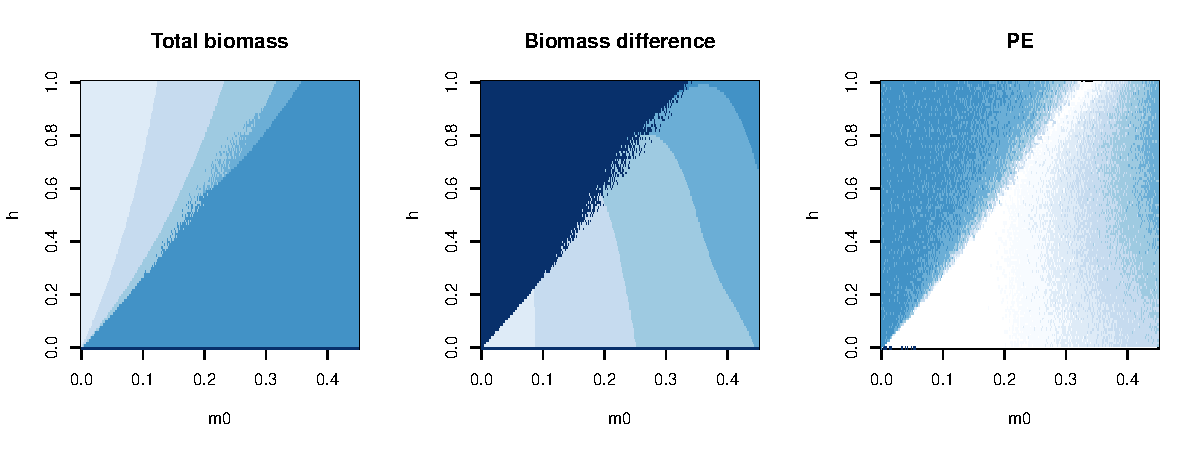
\includegraphics[width=0.8\textwidth]{figs2/fig_MDPE_hm_ddm.pdf}
% \caption{
% The same simulations as presented in Figure \ref{fig:PE}, except with density dependent straying, where $m(t) = m_0\left(1-N(t)/(C+N(t)\right)$. Light colors = high values.
% } \label{fig:ddm}
% \end{figure*}


\end{document}
